% Options for packages loaded elsewhere
\PassOptionsToPackage{unicode}{hyperref}
\PassOptionsToPackage{hyphens}{url}
\documentclass[
]{article}
\usepackage{xcolor}
\usepackage[margin=1in]{geometry}
\usepackage{amsmath,amssymb}
\setcounter{secnumdepth}{-\maxdimen} % remove section numbering
\usepackage{iftex}
\ifPDFTeX
  \usepackage[T1]{fontenc}
  \usepackage[utf8]{inputenc}
  \usepackage{textcomp} % provide euro and other symbols
\else % if luatex or xetex
  \usepackage{unicode-math} % this also loads fontspec
  \defaultfontfeatures{Scale=MatchLowercase}
  \defaultfontfeatures[\rmfamily]{Ligatures=TeX,Scale=1}
\fi
\usepackage{lmodern}
\ifPDFTeX\else
  % xetex/luatex font selection
\fi
% Use upquote if available, for straight quotes in verbatim environments
\IfFileExists{upquote.sty}{\usepackage{upquote}}{}
\IfFileExists{microtype.sty}{% use microtype if available
  \usepackage[]{microtype}
  \UseMicrotypeSet[protrusion]{basicmath} % disable protrusion for tt fonts
}{}
\makeatletter
\@ifundefined{KOMAClassName}{% if non-KOMA class
  \IfFileExists{parskip.sty}{%
    \usepackage{parskip}
  }{% else
    \setlength{\parindent}{0pt}
    \setlength{\parskip}{6pt plus 2pt minus 1pt}}
}{% if KOMA class
  \KOMAoptions{parskip=half}}
\makeatother
\usepackage{longtable,booktabs,array}
\usepackage{calc} % for calculating minipage widths
% Correct order of tables after \paragraph or \subparagraph
\usepackage{etoolbox}
\makeatletter
\patchcmd\longtable{\par}{\if@noskipsec\mbox{}\fi\par}{}{}
\makeatother
% Allow footnotes in longtable head/foot
\IfFileExists{footnotehyper.sty}{\usepackage{footnotehyper}}{\usepackage{footnote}}
\makesavenoteenv{longtable}
\usepackage{graphicx}
\makeatletter
\newsavebox\pandoc@box
\newcommand*\pandocbounded[1]{% scales image to fit in text height/width
  \sbox\pandoc@box{#1}%
  \Gscale@div\@tempa{\textheight}{\dimexpr\ht\pandoc@box+\dp\pandoc@box\relax}%
  \Gscale@div\@tempb{\linewidth}{\wd\pandoc@box}%
  \ifdim\@tempb\p@<\@tempa\p@\let\@tempa\@tempb\fi% select the smaller of both
  \ifdim\@tempa\p@<\p@\scalebox{\@tempa}{\usebox\pandoc@box}%
  \else\usebox{\pandoc@box}%
  \fi%
}
% Set default figure placement to htbp
\def\fps@figure{htbp}
\makeatother
\setlength{\emergencystretch}{3em} % prevent overfull lines
\providecommand{\tightlist}{%
  \setlength{\itemsep}{0pt}\setlength{\parskip}{0pt}}
\usepackage{bookmark}
\IfFileExists{xurl.sty}{\usepackage{xurl}}{} % add URL line breaks if available
\urlstyle{same}
\hypersetup{
  hidelinks,
  pdfcreator={LaTeX via pandoc}}

\author{}
\date{\vspace{-2.5em}}

\begin{document}

\section{S3 · Practicing Qualitative
Methods}\label{s3-practicing-qualitative-methods}

\begin{quote}
\textbf{Source} : \texttt{S3\_PracticingQualitativeMethods.pdf} (9
pages) \textbf{Pages couvertes} : 1--9 ✅ exhaustif \textbf{Statut} : ✅
Complet \textbf{Type} : Session pratique en classe (peu de théorie
nouvelle, beaucoup de logistique projet)
\end{quote}

\begin{center}\rule{0.5\linewidth}{0.5pt}\end{center}

\subsection{🎯 Pourquoi cette session
existe}\label{pourquoi-cette-session-existe}

\begin{quote}
\textbf{Hook} : Tu peux lire pendant des heures comment conduire une
interview, mais tant que tu n'en as pas fait une vraie, tu ne sais pas.
Cette session t'oblige à passer à l'acte, encadré, avant de le faire en
autonomie pour ton projet Matrix.
\end{quote}

\textbf{Idée centrale} : la théorie des méthodes qualitatives (S1) prend
tout son sens quand on la pratique. S3 est la session ``mise en jambes''
: on s'entraîne en classe pour ne pas se planter sur le terrain.

\begin{center}\rule{0.5\linewidth}{0.5pt}\end{center}

\subsection{1. Course Roadmap --- vue d'ensemble du cours {[}slide 2 \&
8{]}}\label{course-roadmap-vue-densemble-du-cours-slide-2-8}

\begin{figure}
\centering
\pandocbounded{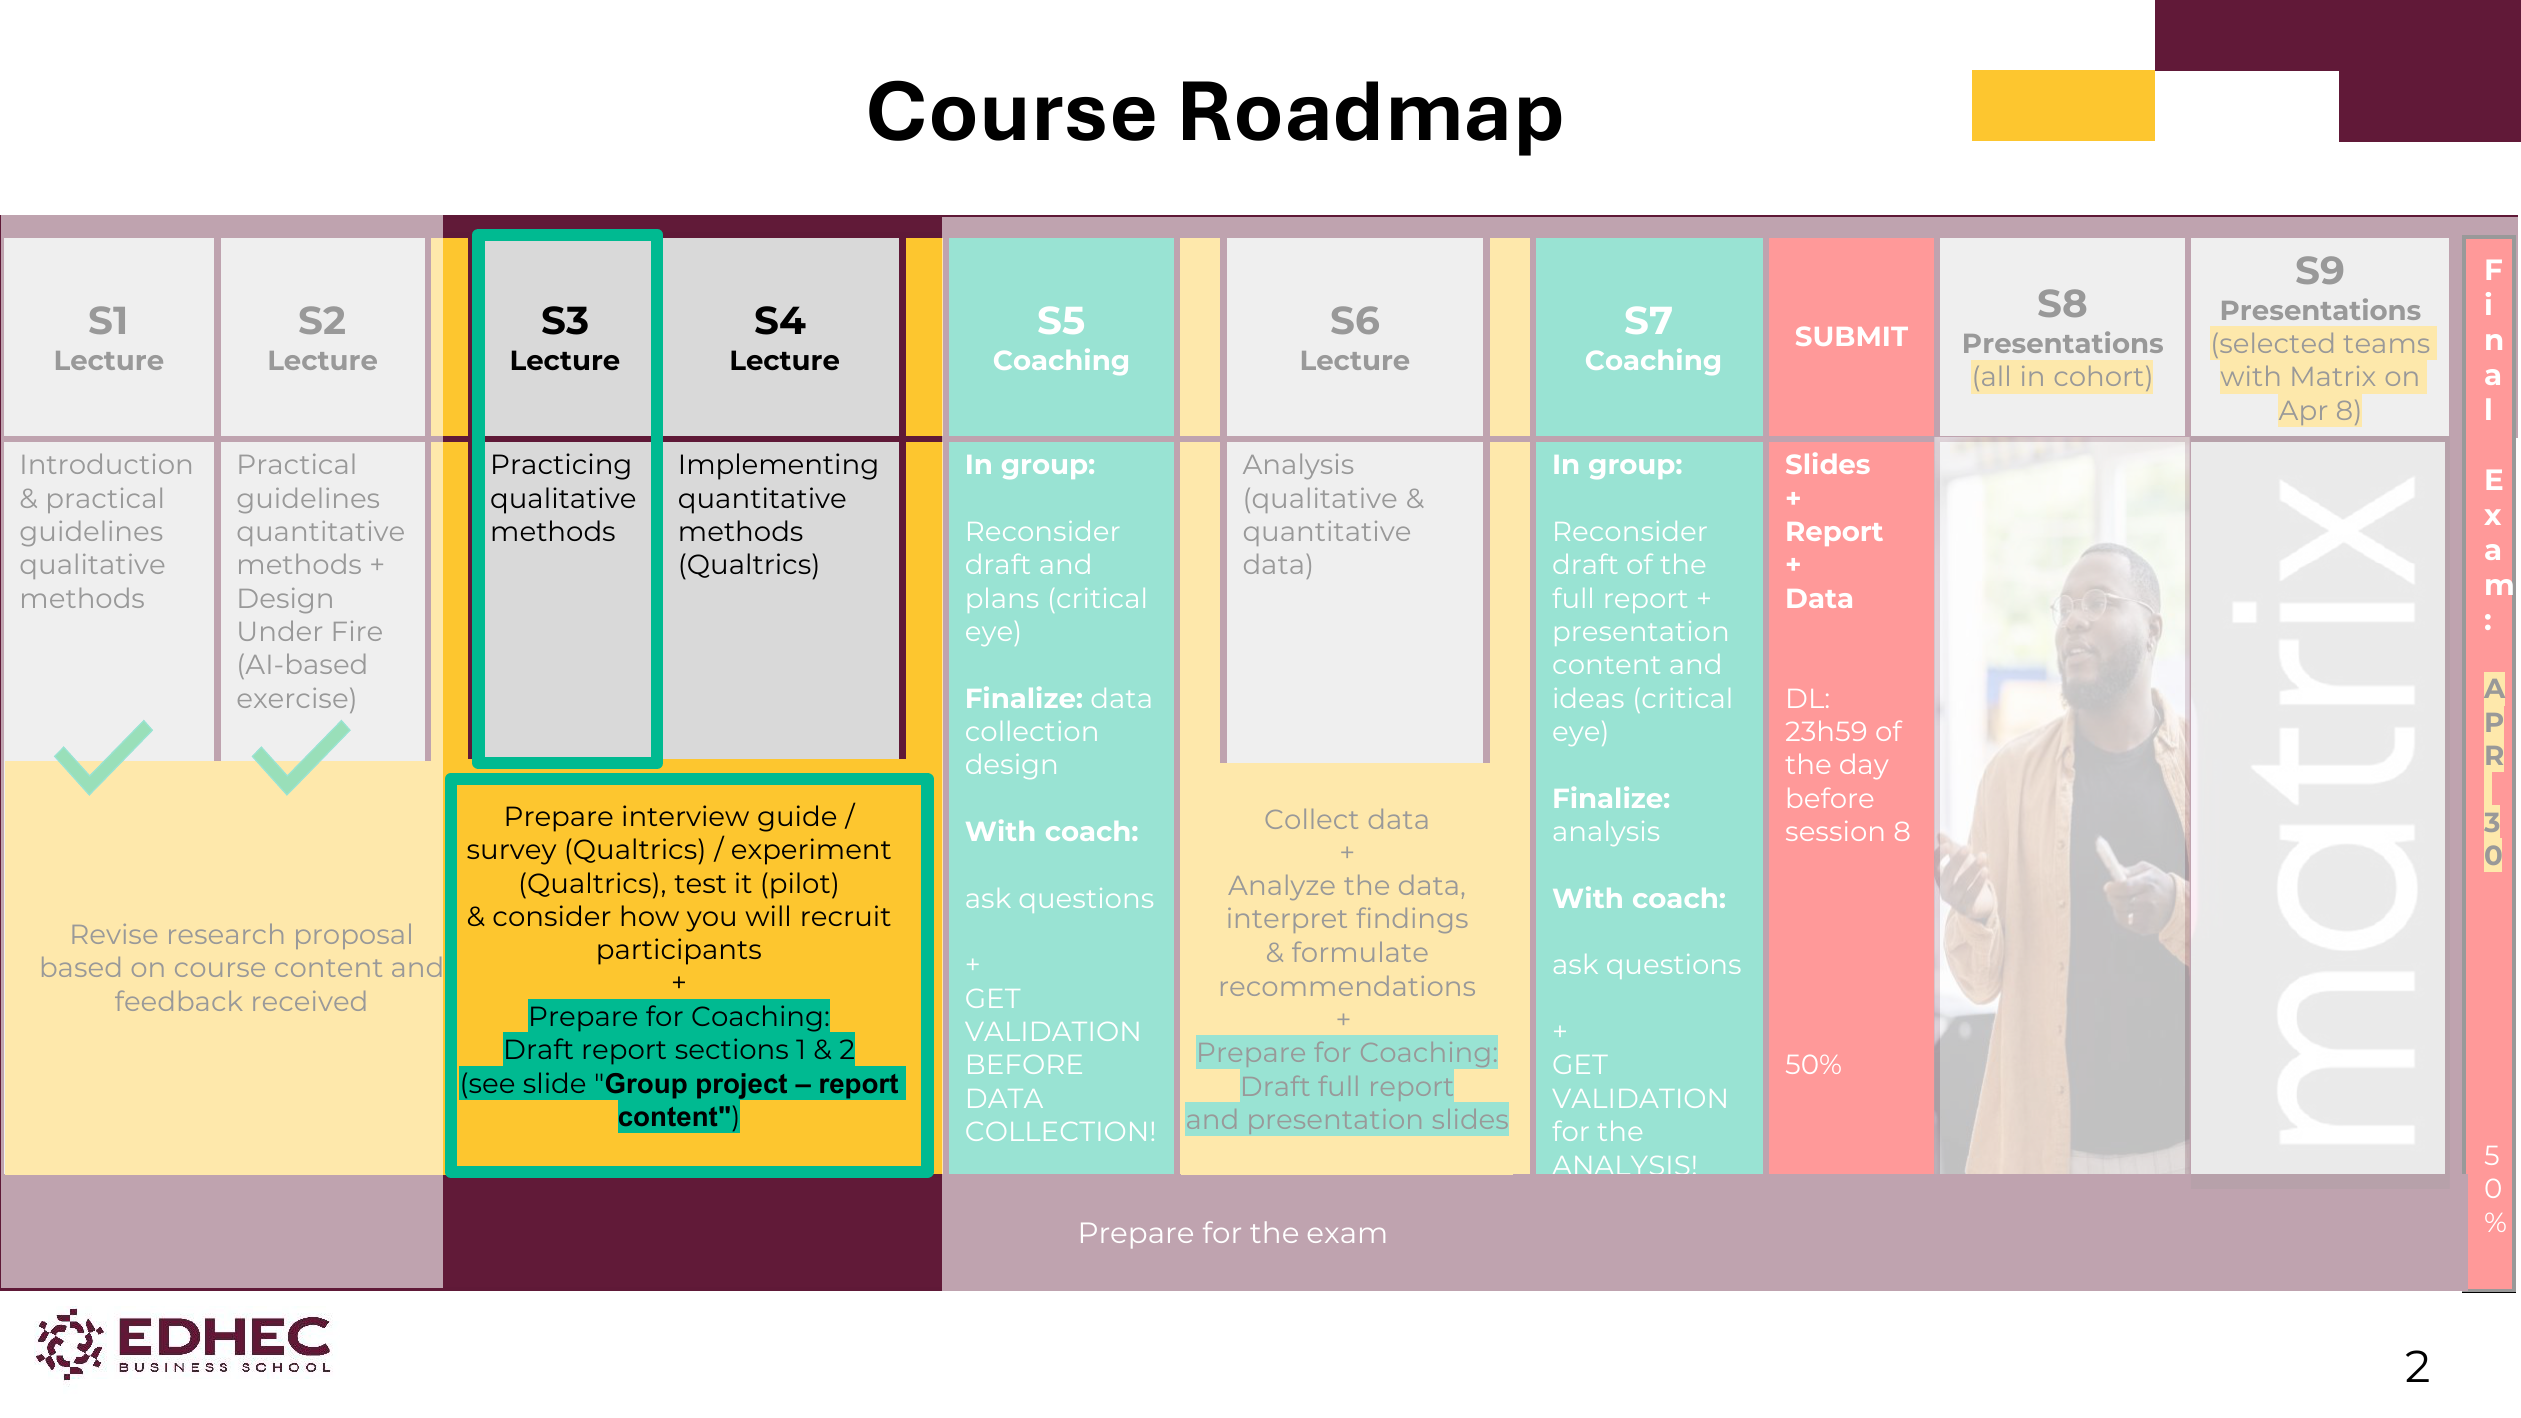
\includegraphics[keepaspectratio]{screens/s3_02_roadmap-2.png}}
\caption{Course Roadmap}
\end{figure}

\subsubsection{À retenir absolument : les deliverables entre chaque
session}\label{uxe0-retenir-absolument-les-deliverables-entre-chaque-session}

\begin{longtable}[]{@{}
  >{\raggedright\arraybackslash}p{(\linewidth - 2\tabcolsep) * \real{0.5000}}
  >{\raggedright\arraybackslash}p{(\linewidth - 2\tabcolsep) * \real{0.5000}}@{}}
\toprule\noalign{}
\begin{minipage}[b]{\linewidth}\raggedright
Période
\end{minipage} & \begin{minipage}[b]{\linewidth}\raggedright
Ce que tu dois préparer
\end{minipage} \\
\midrule\noalign{}
\endhead
\bottomrule\noalign{}
\endlastfoot
\textbf{Avant S3} & Réviser le research proposal selon le contenu du
cours et le feedback reçu \\
\textbf{Avant S4} & Préparer \textbf{interview guide / survey Qualtrics
/ experiment Qualtrics}, faire un \textbf{pilot test}, réfléchir au
\textbf{recrutement des participants}, et \textbf{rédiger les sections 1
\& 2 du rapport} pour le coaching S5 \\
\textbf{Avant S5} & Plan finalisé, prêt pour validation par le coach \\
\textbf{S5 --- Coaching} & ``Critical eye'' sur le draft + finalize data
collection design + \textbf{GET VALIDATION BEFORE DATA COLLECTION} \\
\textbf{Avant S6} & (Rien de neuf, on reçoit le contenu d'analyse) \\
\textbf{Entre S6 et S7} & \textbf{Collecter les données} + analyser +
interpréter + formuler des recommandations + draft full report et
slides \\
\textbf{S7 --- Coaching} & ``Critical eye'' sur le rapport complet +
\textbf{GET VALIDATION FOR THE ANALYSIS} \\
\textbf{SUBMIT} & Slides + Report + Data, \textbf{deadline 23h59 la
veille de S8} \\
\textbf{S8} & Présentations toute la cohorte \\
\textbf{S9} & Présentations sélectionnées devant \textbf{Matrix} (le 8
avril) \\
\textbf{30 avril} & \textbf{Examen final} (50\% de la note) \\
\end{longtable}

\begin{quote}
\textbf{💡 Intuition} : le cours a deux temps. \textbf{Avant S6} = tu
prépares ton dispositif (sans collecter). \textbf{Après S6} = tu
collectes et analyses. Tu ne dois JAMAIS commencer la collecte sans la
validation du coach en S5.
\end{quote}

\begin{quote}
\textbf{⚠️ Piège} : commencer à collecter les données avant d'avoir reçu
la validation S5 = risque énorme de devoir tout refaire. Le coaching
n'est pas optionnel.
\end{quote}

\begin{center}\rule{0.5\linewidth}{0.5pt}\end{center}

\subsection{2. Outils à installer {[}slide
3{]}}\label{outils-uxe0-installer-slide-3}

\begin{longtable}[]{@{}
  >{\raggedright\arraybackslash}p{(\linewidth - 4\tabcolsep) * \real{0.3333}}
  >{\raggedright\arraybackslash}p{(\linewidth - 4\tabcolsep) * \real{0.3333}}
  >{\raggedright\arraybackslash}p{(\linewidth - 4\tabcolsep) * \real{0.3333}}@{}}
\toprule\noalign{}
\begin{minipage}[b]{\linewidth}\raggedright
Outil
\end{minipage} & \begin{minipage}[b]{\linewidth}\raggedright
Pour quoi
\end{minipage} & \begin{minipage}[b]{\linewidth}\raggedright
Quand
\end{minipage} \\
\midrule\noalign{}
\endhead
\bottomrule\noalign{}
\endlastfoot
\textbf{Qualtrics} & Surveys + designs expérimentaux & \textbf{ASAP}
(dès maintenant) \\
\textbf{SPSS} & Analyse quantitative & Avant la \textbf{Session 6} \\
\textbf{Taguette} & Codage qualitatif & Avant la \textbf{Session 6} \\
\end{longtable}

\begin{quote}
\textbf{🎯 Action concrète} : si tu ne l'as pas encore fait, va sur
Blackboard, rubrique \textbf{``Tools file on BB''}, et installe les 3.
\end{quote}

\begin{center}\rule{0.5\linewidth}{0.5pt}\end{center}

\subsection{3. Part 1 --- Pratique d'interviews {[}slide
4{]}}\label{part-1-pratique-dinterviews-slide-4}

\begin{figure}
\centering
\pandocbounded{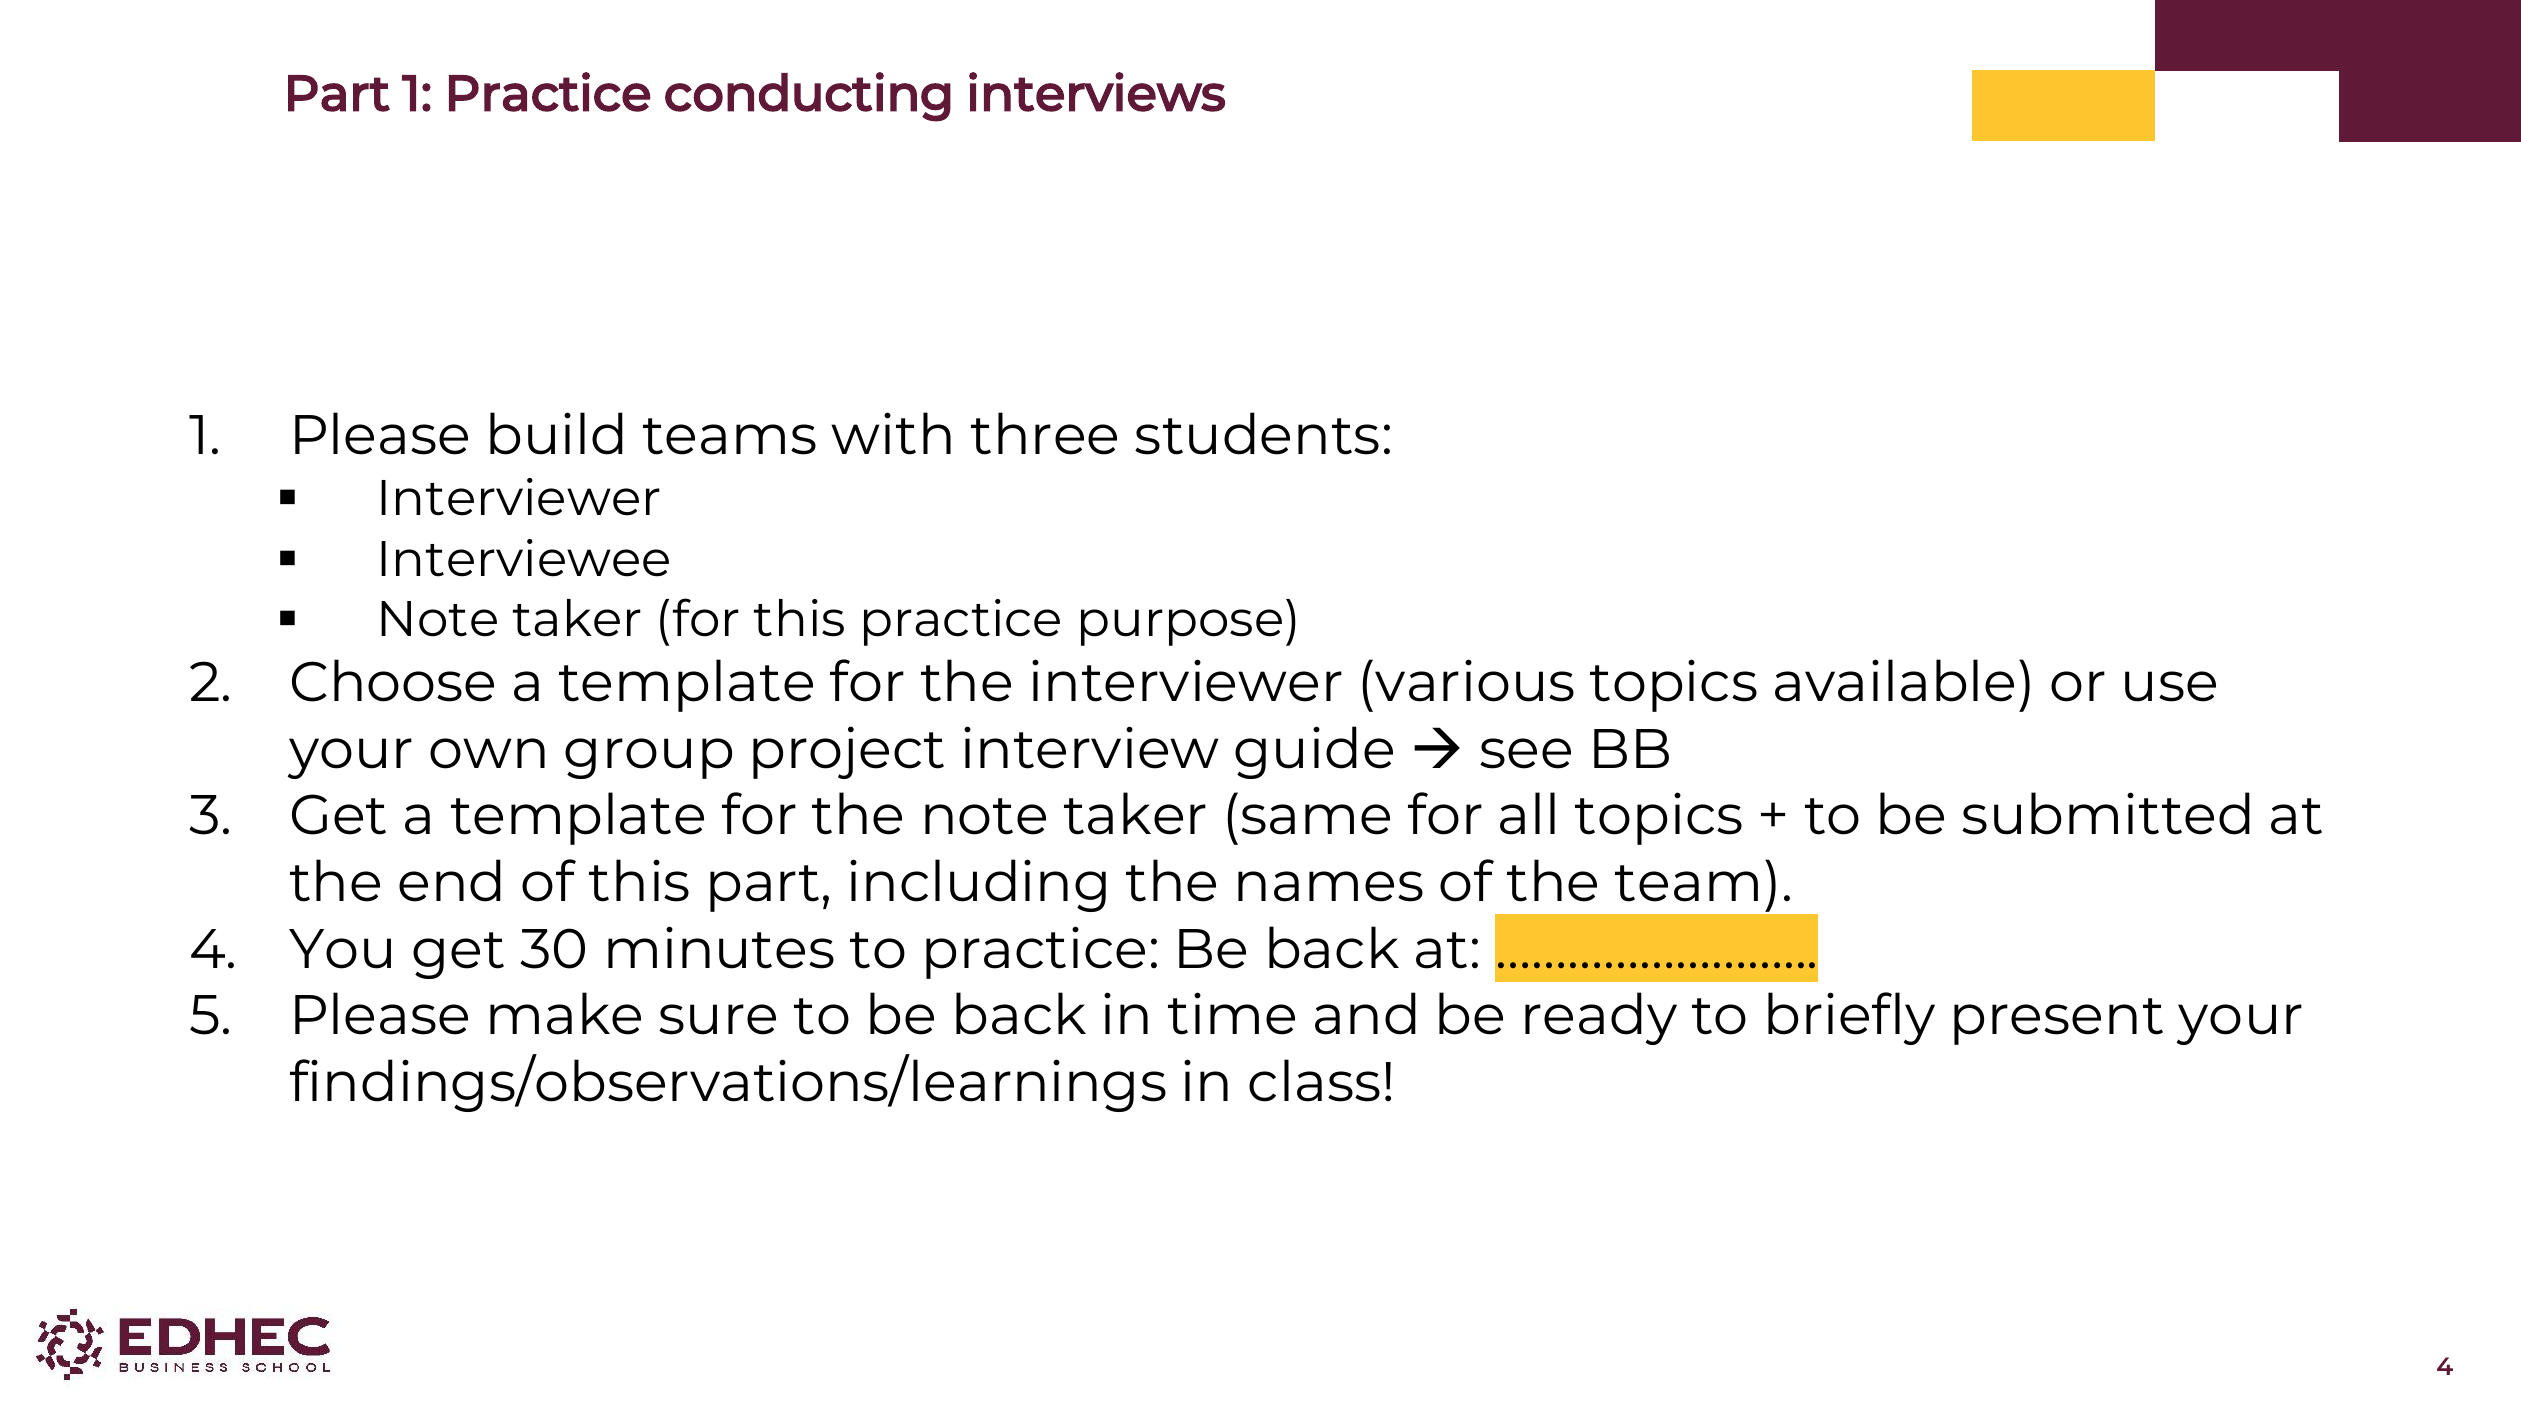
\includegraphics[keepaspectratio]{screens/s3_04_part1-4.png}}
\caption{Instructions Part 1}
\end{figure}

\subsubsection{Setup}\label{setup}

\begin{itemize}
\tightlist
\item
  \textbf{Équipes de 3 étudiants} :

  \begin{itemize}
  \tightlist
  \item
    1 \textbf{Interviewer}
  \item
    1 \textbf{Interviewee}
  \item
    1 \textbf{Note taker} (pour cette session uniquement, pas dans la
    vraie vie)
  \end{itemize}
\item
  Choisir un \textbf{template} d'interviewer (plusieurs sujets dispo sur
  BB) OU utiliser le \textbf{guide d'interview de votre projet}
\item
  Récupérer le template de \textbf{note taker} (identique pour tous, à
  rendre à la fin avec les noms de l'équipe)
\item
  \textbf{30 minutes} chrono
\item
  Être prêt à présenter brièvement vos observations/learnings en classe
\end{itemize}

\subsubsection{Pourquoi un note taker en pratique seulement
?}\label{pourquoi-un-note-taker-en-pratique-seulement}

\begin{quote}
\textbf{💡 Intuition} : sur le terrain, tu enregistres l'audio (avec
consentement) et tu retranscris ensuite. Un note taker en plus n'est pas
standard --- mais ici, il sert à observer la dynamique pour donner du
feedback à l'interviewer.
\end{quote}

\begin{center}\rule{0.5\linewidth}{0.5pt}\end{center}

\subsection{4. Part 2 --- Pratique de focus groups {[}slide
6{]}}\label{part-2-pratique-de-focus-groups-slide-6}

\begin{figure}
\centering
\pandocbounded{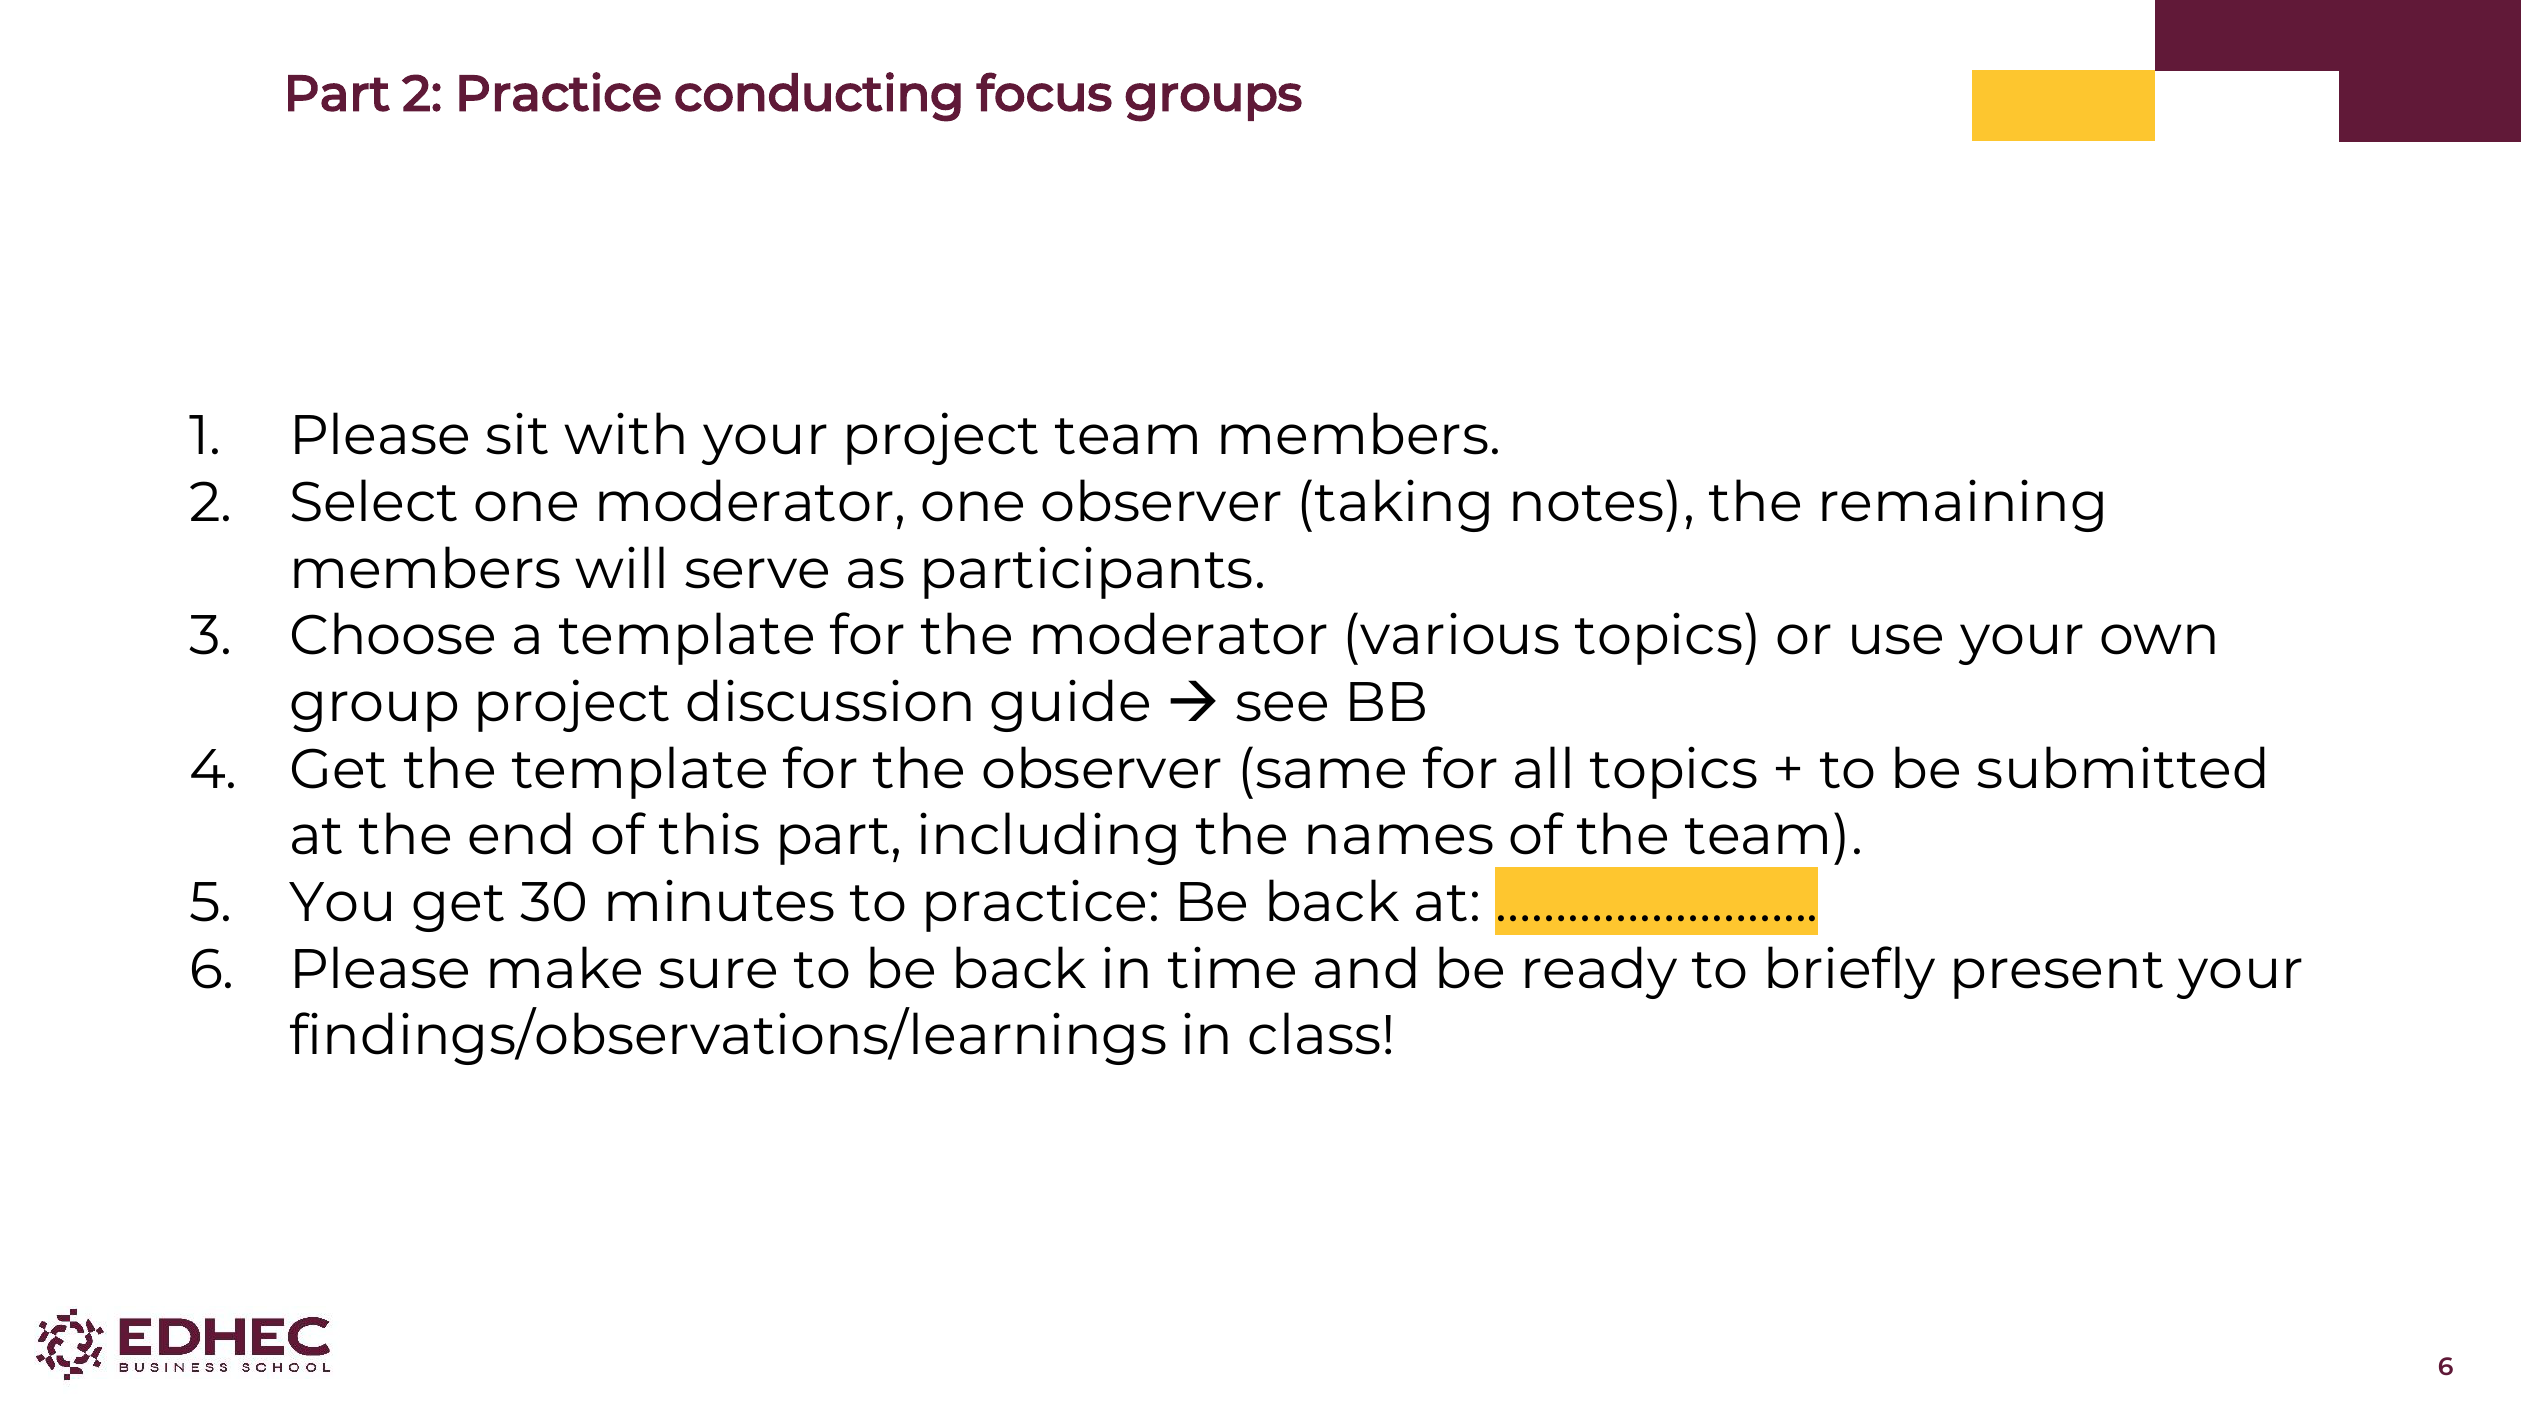
\includegraphics[keepaspectratio]{screens/s3_06_part2-6.png}}
\caption{Instructions Part 2}
\end{figure}

\subsubsection{Setup}\label{setup-1}

\begin{itemize}
\tightlist
\item
  \textbf{S'asseoir avec votre équipe projet Matrix}
\item
  Distribuer les rôles :

  \begin{itemize}
  \tightlist
  \item
    \textbf{1 modérateur} (mène la discussion)
  \item
    \textbf{1 observateur} (prend des notes sur la dynamique de groupe)
  \item
    \textbf{Le reste} = participants
  \end{itemize}
\item
  Choisir un template de modérateur OU utiliser le \textbf{discussion
  guide de votre projet}
\item
  Récupérer le template d'\textbf{observateur} (identique pour tous, à
  rendre à la fin)
\item
  \textbf{30 minutes} chrono
\item
  Présentation brève en classe
\end{itemize}

\subsubsection{Différence rôle modérateur vs
observateur}\label{diffuxe9rence-ruxf4le-moduxe9rateur-vs-observateur}

\begin{quote}
\textbf{💡 Intuition} : le modérateur fait parler le groupe et gère le
temps. L'observateur ne parle pas --- il regarde qui prend la parole,
qui se tait, comment les opinions se forment. Les deux rôles sont
complémentaires.
\end{quote}

\begin{center}\rule{0.5\linewidth}{0.5pt}\end{center}

\subsection{✅ Test toi sur S3}\label{test-toi-sur-s3}

\textbf{Q1} --- Tu finalises ton plan de collecte de données. Tu peux
commencer à recruter des participants ?

\begin{quote}
\textbf{Réponse} : \textbf{Non, pas avant la validation du coach en S5.}
``GET VALIDATION BEFORE DATA COLLECTION'' est explicite dans la roadmap.
\end{quote}

\textbf{Q2} --- Quels sont les 3 rôles dans la pratique d'interview en
S3 ?

\begin{quote}
\textbf{Réponse} : Interviewer, Interviewee, \textbf{Note taker}. (Le
note taker est spécifique à cette session pratique --- il n'existe pas
dans une vraie interview où on enregistre.)
\end{quote}

\textbf{Q3} --- Quelle est la deadline pour soumettre slides + report +
data ?

\begin{quote}
\textbf{Réponse} : \textbf{23h59 la veille de la Session 8.} Pas le jour
J de S8.
\end{quote}

\textbf{Q4} --- Avant S4, qu'est-ce que tu dois avoir préparé ?

\begin{quote}
\textbf{Réponse} : (1) interview guide / survey Qualtrics / experiment
Qualtrics, (2) \textbf{pilot test} réalisé, (3) plan de
\textbf{recrutement des participants}, (4) draft des sections 1 \& 2 du
rapport.
\end{quote}

\begin{center}\rule{0.5\linewidth}{0.5pt}\end{center}

\subsection{🎓 Points d'examen potentiels (probabilité faible mais à
connaître)}\label{points-dexamen-potentiels-probabilituxe9-faible-mais-uxe0-connauxeetre}

S3 étant une session pratique, peu de questions de cours probables. Mais
: - Les \textbf{3 outils du cours} (Qualtrics, SPSS, Taguette) --- peut
être demandé ``lequel pour quoi'' - La \textbf{différence entre
modérateur et observateur} dans un focus group - Le \textbf{rôle du
pilot test} avant la collecte (concept à connaître pour S2 et S4)

\begin{center}\rule{0.5\linewidth}{0.5pt}\end{center}

\subsection{📚 Références}\label{ruxe9fuxe9rences}

\begin{itemize}
\tightlist
\item
  EDHEC Marketing Research Methods, Session 3 slides (2026)
\item
  Tools file on Blackboard
\end{itemize}

\begin{center}\rule{0.5\linewidth}{0.5pt}\end{center}

\subsection{⚠️ À vérifier}\label{uxe0-vuxe9rifier}

\begin{itemize}
\tightlist
\item
  Aucune ambiguïté détectée dans les 9 slides.
\end{itemize}

\end{document}
